%!TeX program = xelatex
\documentclass[12pt,hyperref,a4paper,UTF8]{ctexart}
% 页面设置（符合规范：上30mm，下25mm，左30mm，右20mm）
\usepackage[a4paper, top=30mm, bottom=25mm, left=30mm, right=20mm]{geometry}
\usepackage{listings}
\usepackage{xcolor}
\usepackage{setspace}
\setstretch{1.5}             % 全局行距1.5倍

\usepackage{graphicx} 

% 算法宏包
\usepackage[ruled,linesnumbered]{algorithm2e}
\SetAlgorithmName{算法}{算法}{算法列表}
\SetKwInput{KwIn}{输入}
\SetKwInput{KwOut}{输出}
\SetKwProg{Fn}{函数}{：}{}
\newtheorem{example}{例}[section]
\newtheorem{remark}{注}[section]
\SetKwComment{tcp}{//}{}

\usepackage{amsmath,amssymb}
\newcommand{\R}{\mathbb{R}}
\newcommand{\A}{\mathcal{A}}
\newcommand{\V}{\mathcal{V}}
\newcommand{\E}{\mathcal{E}}
\newcommand{\X}{\mathcal{X}}
\DeclareMathOperator{\Dist}{Dist}
\newcommand{\N}{\mathbb{N}}
\DeclareMathOperator*{\argmin}{arg\,min}

% 定理环境
\newtheorem{definition}{定义}[section]
\newtheorem{theorem}{定理}[section]
\newtheorem{lemma}{引理}[section]
\newtheorem{assumption}{假设}[section]
\newtheorem{corollary}{推论}[section]
\newtheorem{proposition}{命题}[section]

% 公式、图、表按章编号
\usepackage{amsmath}
\numberwithin{equation}{section}
\numberwithin{figure}{section}
\numberwithin{table}{section}

% 图表标题字体设置（符合规范：表题5号黑体加粗，图题5号宋体）
\usepackage{caption}
\captionsetup[table]{font={bf,small},labelsep=space,skip=2pt,aboveskip=2pt}
\captionsetup[figure]{font={small,rm},labelsep=space,skip=2pt,aboveskip=2pt}
\renewcommand{\tablename}{表}
\renewcommand{\figurename}{图}

% 上标引用（符合规范：引用序号置于右上角）
\usepackage{cite}
\renewcommand{\citeleft}{[}
\renewcommand{\citeright}{]}

% 页眉页码（正文页眉右侧阿拉伯数字页码，摘要目录罗马数字）
\usepackage{fancyhdr}
\pagestyle{fancy}
\fancyhf{}
\fancyhead[R]{\thepage}
\renewcommand{\headrulewidth}{0pt}

% 章节标题格式（符合规范）
\usepackage{titlesec}
% \titleclass{\section}{top}   % 每章另起一页，避免使用\let\old@section
\titleformat{\section}
  {\centering\heiti\zihao{3}}{\thesection}{1em}{}
\titlespacing*{\section}{0pt}{20pt}{20pt}
\titleformat{\subsection}
  {\heiti\zihao{-4}}{\thesubsection}{1em}{}
\titlespacing*{\subsection}{0pt}{0.5\baselineskip}{0.5\baselineskip}
\titleformat{\subsubsection}
  {\heiti\zihao{-4}}{\thesubsubsection}{1em}{}
\titlespacing*{\subsubsection}{0pt}{0.5\baselineskip}{0.5\baselineskip}

% 正文默认字体：小四号宋体
\renewcommand{\normalsize}{\zihao{-4}}
\setlength{\parindent}{2em}   % 首行缩进2字符

% 英文数字默认Times New Roman
\setmainfont{Times New Roman}

% 表格内文字为5号宋体，开放式表格（无竖线）
\usepackage{booktabs}
\let\oldtabular\tabular
\renewenvironment{tabular}{\small\oldtabular}{}

% 附录编号设置（图、表、公式以附录字母开头）
\usepackage{appendix}
\renewcommand{\appendixname}{附录}
\renewcommand{\appendixpagename}{附录}
\renewcommand{\appendixtocname}{附录}

% hyperref 放在最后
\usepackage[colorlinks=true,linkcolor=blue,citecolor=blue]{hyperref}

% 列表间距调整
\usepackage{enumitem}
\setlist[itemize]{itemsep=0pt, parsep=0pt}

\begin{document}

%% 手动封面页（确保日期不溢出）
\begin{titlepage}
    \centering
    \vspace*{2cm}
    {\heiti\Huge 计算机科学研究方法论课程报告}\\[1.5cm]
    {\heiti\Large Byzantine-Resilient Multiagent Optimization}\\[4cm]
    
    {\kaishu\Large 学院：计算机学院}\\[1cm]
    {\kaishu\Large 专业：计算机科学与技术}\\[1cm]
    {\kaishu\Large 学号：23371355}\\[1cm]
    {\kaishu\Large 姓名：王梓恒}\\[1cm]
    
    \vfill
    {\kaishu\Large 2026年5月21日}
\end{titlepage}
\clearpage

%% 摘要页（罗马数字页码）
\pagenumbering{Roman}
\setcounter{page}{1}

\begin{center}
    {\heiti\zihao{-3} 拜占庭容错的多智能体优化} \\[2ex]   % 论文题目小3黑体
    {\heiti\zihao{3} 摘要} \\[2ex]                         % “摘要”3号黑体
    {\normalfont\zihao{-4} 学生：王梓恒 \qquad 指导教师：刘雪峰} \\[2ex]  % 请替换实际姓名
\end{center}

\noindent \quad \quad  分布式多智能体优化旨在通过无中心节点间的局部协作，最小化所有节点局部代价函数的算术平均值目标。然而，传统的算术平均优化目标在面临拜占庭故障时很脆弱，使得哪怕单一的恶意节点也能通过注入极端或不一致数据完全操控全局的优化结果。为了解决该问题，本文重构全局目标为仅由正常节点局部函数构成的凸组合。为了防止正常节点的数据权重被恶意节点稀释，本文首次提出了($\beta, \gamma$)-可容许性这一数学度量，用于限制正常节点占比不小于$\beta$的个数不小于$\gamma$。此外，本文通过聚焦标量局部代价函数，迈出了解决所提出的拜占庭容错多智能体优化问题的第一步。本文的研究结果可为一般化的局部代价函数提供有用的见解。

\vspace{1\baselineskip}
\noindent {\heiti\zihao{4} 关键词}：{\zihao{-4} 计算与人工智能，容错性，容错控制，机器学习/分布式计算，可靠性}

\newpage
%% 目录页（罗马数字页码，无页眉）
\tableofcontents
\thispagestyle{plain}

%% 正文开始（阿拉伯数字页码，页眉右侧页码）
\newpage
\pagenumbering{arabic}
\setcounter{page}{1}
\pagestyle{fancy}

\section{引言}

\quad \quad  在网络化的多智能体系统中，分布式协作优化是一个不可或缺的核心任务。在理想的无对抗网络环境中，多智能体优化的标准范式是假设网络中的每个智能体持有一个局部代价函数，随后所有的智能体通过点对点的局部通信相互协作，共同寻找一个能够最小化全体局部代价函数算术平均值的全局最优解\cite{nedic2009distributed}。这一基于算术平均的协同寻优框架在过去十几年中推动了传感器网络、分布式控制等领域的蓬勃发展，并在理论上得到了充分且成熟的研究。

然而，现实的分布式计算环境极易遭受恶意攻击，现有的基于算术平均值的多智能体优化范式在面临拜占庭故障时存在致命的脆弱性。在拜占庭模型中\cite{lynch1996distributed}，未知子集的智能体可能表现出任意的对抗性行为，甚至向不同的邻居发送自相矛盾的虚假信息。由于算术平均值对极端异常数据没有任何抵抗力，即使网络中仅存在单一的拜占庭节点，它也能完全劫持并摧毁整个多智能体网络的全局优化进程\cite{sundaram2019distributed}。此外，现有的容错一致性算法无法处理梯度寻优\cite{vaidya2012iterative}，而容错机器学习算法又高度依赖数据独立同分布假设及中心化服务器\cite{yin2018byzantine}，导致前人方法均无法直接解决无中心、数据非独立同分布场景下的拜占庭优化难题。

针对上述问题，本文在无中心协调器的前提下，提出了一种全新的拜占庭容错多智能体优化问题框架。为了减少恶意节点对优化结果的干扰，我们摒弃了传统的平均值目标，在数学上将安全的全局优化目标重新界定为仅由正常节点局部代价函数构成的凸组合。更为关键的是，为了防止该凸组合坍缩为只受极少数正常节点主导的结果，我们创新性地引入了($\beta, \gamma$)-可容许性这一严格的数学度量，明确要求最终的全局决策必须至少包含$\gamma$个正常节点的信息，且被采纳的每个正常节点数据的权重占比不得低于$\beta$。

在确立了该合法目标的结构性约束后，我们进一步从理论底层探索了该问题的数学极限，并设计了相应的求解算法。首先，通过不可区分性论证，我们证明了在允许拜占庭节点发送不一致消息的网络中，存在一个不可逾越的不可能性边界。其次，为了逼近这一底线，我们提出了一种基于双重修剪的分布式梯度下降算法。该算法摒弃了单一的状态聚合，转而在局部状态估计和局部梯度计算两个维度上同时引入基于排序的修剪过滤机制，从而有效抵御了多维度的对抗性攻击。

理论分析与收敛性证明表明，本文提出的算法能够确保所有正常智能体的局部估计值渐近收敛到满足($\beta, \gamma$)-可容许性的合法最优解$\mathcal{X}(\beta, \gamma)$集合中。特别地，当底层通信网络为完全图时，该算法所能保证的$\gamma$值完美匹配了不可能性定理中的理论上限，且其实现的$\beta$值达到了理论最优值的$\frac{1}{2}$。这标志着在最恶劣的拜占庭环境下，系统依然能在理论极限附近守住正常节点的协同权益。

综上所述，本文的核心贡献在于：
\begin{itemize}
    \item 提出了一种无中心拜占庭容错多智能体优化框架，并首创了($\beta, \gamma$)-可容许性度量，以严格刻画和约束容错全局目标的凸系数结构。
    \item 通过证明该优化问题的不可能性定理，确立了任何分布式算法在防范拜占庭攻击时所能达到的理论上限。
    \item 提出了一种基于双重修剪的分布式梯度下降算法，并严格证明了其在完全图网络中能够达到与理论极限相匹配的最优容错性能。
\end{itemize}

\section{相关工作}

\quad \quad  针对拜占庭容错多智能体协作的研究背景，前期的探索主要集中在以下三个方面。通过分析这些工作的模型设定与处理机制，可以明确在去中心化优化的背景下引入局部代价函数所面临的种种挑战。

\subsection{基于约简机制的鲁棒迭代一致性}

\quad \quad  在对抗环境下的分布式协作中，确保正常节点状态的稳定收敛是首要任务。Vaidya等人在其 2012 年的技术报告中，针对点对点通信模型下的任意有向图，深入探讨了迭代式近似共识的理论边界~\cite{vaidya2012iterative}。该工作通过引入修剪算子——即在节点接收到的状态序列中，排序并严格剔除最大与最小的 $f$ 个值（其中常数 $f$ 代表系统预设的全网拜占庭节点数量上限）——有效地屏蔽了恶意节点通过非一致性攻击注入的伪造数据。该研究从数学上确立了约简图（即从原通信图中移除所有可能的故障节点以及正常节点至多 $f$ 条入边后残存的子图）必须满足包含非空源组件的充分必要条件，为后续处理状态偏差提供了拓扑分析框架。

与此同时，LeBlanc等人在早期工作中提出了一类基于子序列约简的鲁棒迭代算法~\cite{leblanc2012consensus}。该算法的核心机理在于要求各节点在聚合信息前，主动忽略那些显著偏离自身当前状态的极端观测值，从而保障系统的渐近一致性。为了对网络的抗干扰能力进行量化，该研究定义了基于拓扑凝聚力的 $(r, s)$-鲁棒性指标。在数学上，该指标要求网络中任意两个不相交且大小不超过 $s$（即局部最多受破坏的节点数）的节点集合，至少有一个集合包含这样的节点：其在自身集合之外拥有至少 $r$ 个邻居（即确保正常节点保留足够多的可靠信息源）。然而，此类工作由于仅针对静态的标量或向量状态进行分析，并未涉及局部输入为成本函数时的梯度更新逻辑，无法直接处理分布式的连续寻优任务。

\subsection{广播模型下的分布式函数计算}

\quad \quad  针对更为复杂的计算任务，部分研究聚焦于在对抗网络中执行特定的函数映射。Sundaram和Hadjicostis提出了一种基于线性迭代策略的分布式函数计算方案，旨在使各节点协作计算出如算术平均值或多项式函数等特定的全局目标~\cite{sundaram2011distributed}。该工作的一个关键假设是采用了广播通信模型，即物理层确保每个节点发送的信息对于其所有入度邻居是完全一致的。这种物理层约束极大限制了拜占庭节点的对抗空间，使其无法针对不同邻居实施具有欺骗性的不一致信息注入。

进一步的理论推导表明，在广播模型假定下，只要网络的顶点连通度(记为 $\kappa$)满足 $\kappa \ge 2f+1$（其中 $f$ 为网络中存在的恶意节点总数），系统即可通过维护状态的历史序列实现对全局函数的精确重构。这里的 $\kappa \ge 2f+1$ 意味着任意两个正常节点之间至少存在 $2f+1$ 条节点不相交的独立路径，从而利用多数表决机制滤除最多 $f$ 条路径上的污染。然而，这种方案的有效性高度依赖于底层协议提供的通信一致性，在通用的点对点网络环境中，广播特性往往难以获得保障。此外，如何在不具备物理层过滤的前提下处理优化过程中由异构局部函数产生的梯度偏差，仍是当前分布式寻优领域亟待攻克的理论难题。

\subsection{局部有界故障模型下的协作分析}

\quad \quad  在探讨故障规模对系统性能的影响时，研究者提出了不同于全局数量限制的故障建模方法。Zhang和Sundaram探讨了信息扩散算法在局部有界故障模型下的鲁棒性~\cite{6315661}。在数学表达上，若记正常节点 $i$ 的邻居集合为 $\mathcal{N}_i$，全网拜占庭节点集合为 $\mathcal{A}$，该模型严格约束 $|\mathcal{N}_i \cap \mathcal{A}| \le f$。即假设在任何正常节点的局部邻域内，遭受拜占庭故障的节点数量均不超过预设常数 $f$，而非像传统模型那样仅对全网故障总数施加全局约束（$|\mathcal{A}| \le b$）。这种建模方式能够更准确地刻画超大规模网络中攻击行为的物理分布特性，并据此推导出了实现信息扩散的边界拓扑条件。

尽管局部故障模型简化了大规模拓扑下攻击的复杂度分析，但在实际的分布式优化应用中，算法通常仍需在更具一般性的全局故障模型下保持稳健。此外，现有关于局部故障模型的研究多侧重于信息的扩散速率与拓扑覆盖范围，尚未充分探讨在数据非独立同分布条件下，如何通过严格的数学约束（例如为正常节点分配非平凡的凸系数权重）来防止全局决策被极端观测值或伪装的对抗数据所劫持。因此，在构建具备结构性保护机制的容错优化框架方面，仍存在显著的理论探索空间。

\section{系统概述}

\quad \quad  在无对抗网络中，多智能体分布式优化的经典范式是所有节点通过交换局部状态与梯度信息，协同最小化所有局部代价函数的算术平均值\cite{nedic2009distributed} 
\begin{equation}
\frac{1}{n}\sum_{i=1}^{n} f_i(x) 
\label{average value}
\end{equation}其中，$x \in \mathbb{R}^d$ 为全局决策变量，$f_i(x): \mathbb{R}^d \to \mathbb{R}$ 代表节点 $i$ 的局部可容许成本函数，而$n$ 为网络中总的节点个数。这一基于算术平均的聚合机制赋予了所有节点完全平等的权重（即每个节点的权重均为$\frac{1}{n}$），构成了分布式优化中广泛采用的基线方法。

然而，在面临拜占庭故障时，该基线方法显现出明显的局限性。由于算术平均算子对极端异常值缺乏鲁棒性，网络中即使仅存在少数的拜占庭节点，也可通过在通信中注入趋于无穷大的伪造状态或异常梯度值，导致聚合后的全局最优解发生任意偏移，进而使得整个优化系统无法收敛。

为了克服上述缺陷，本文在理论框架上对优化目标进行了重构。如图 \ref{fig:example} 所示，系统在宏观上转换为约束诚实智能体协同最小化一个仅由诚实节点局部代价函数构成的凸组合，即
\begin{equation}
\min \sum_{i \in \mathcal{V} \setminus \mathcal{A}} \alpha_i f_i(x)
\label{new_target}
\end{equation}
在公式\ref{new_target}中，$\mathcal{V} = \{1, 2, \dots, n\}$ 表示网络中所有节点的集合，$\mathcal{A}$ 代表遭受拜占庭故障的对抗节点集合，$\mathcal{V} \setminus \mathcal{A}$ 即为诚实节点的集合；$\alpha_i \ge 0$ 且满足 $\sum_{i \in \mathcal{V} \setminus \mathcal{A}} \alpha_i = 1$，代表诚实节点 $i$ 在最终全局决策中所占的实际权重。

为避免上述凸组合塌缩为由极个别诚实节点主导的平凡解，本文进一步引入了 ($\beta, \gamma$)-可容许性约束。该约束在数学上要求诚实节点集合中，必须至少有 $\gamma$ 个节点的权重 $\alpha_i$ 大于或等于预设的下界 $\beta$。这一机制确保了足够数量的诚实节点在全局决策中保持有效的影响力。

为求解该重构目标，本文提出了一种基于双重修剪的分布式梯度下降算法。该算法通过在局部状态估计和局部梯度计算两个维度上同时执行极值截断操作，将含有对抗注入的非线性状态演化等效地约束在诚实节点的凸包内部。理论分析表明，在确保通信图满足约简图连通假设的前提下，该方法能够在牺牲一定寻优精度的条件下，保障系统在对抗环境中向合法目标解集渐近收敛。

\begin{figure}[h]
    \centering
    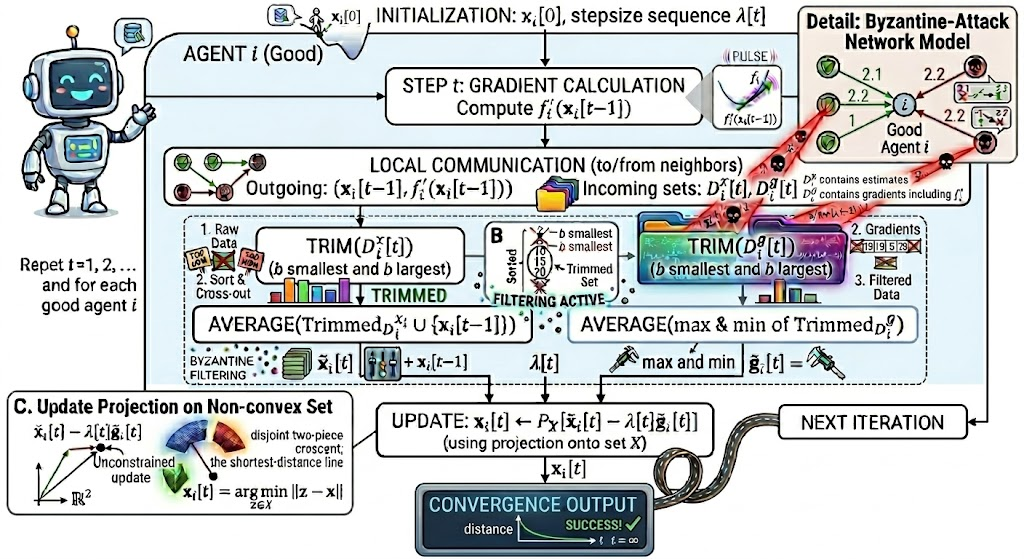
\includegraphics[width=0.8\textwidth]{function.jpg}
    \caption{多智能体系统的交互与网络模型示意图}
    \label{fig:example}
\end{figure}

\section{问题描述}

\subsection{网络与故障模型}
\quad \quad  多智能体网络由 $n$ 个通过有向通信图 $G(\mathcal{V},\mathcal{E})$ 交互的智能体节点组成，其中 $\mathcal{V} = \{1,\ldots,n\}$ 表示节点集合，$\mathcal{E}$ 表示边集合。网络中存在一个未知的智能体子集 $\mathcal{A}$ 遭受拜占庭故障。设定 $|\mathcal{A}| \le b$，其中 $b$ 为网络中所能容忍的最大拜占庭节点个数。记 $\phi \triangleq |\mathcal{A}|$，则满足 $\phi \le b$。本文限定总节点数 $n \ge 3b+1$。

令 $\mathcal{N}_i$ 为智能体 $i$ 的入度邻居集合，$d_i \triangleq |\mathcal{N}_i|$ 为其入度。每个智能体可向自身发送消息，但为了符号表述严谨，集合 $\mathcal{E}$ 中不包含自环即 $(i,i)\notin\mathcal{E}$。

本文采用标准拜占庭故障模型刻画系统威胁 \cite{lynch1996distributed}。该模型假定对抗节点具备完全的网络信息，包括拓扑结构、诚实节点的局部程序及当前状态。拜占庭智能体可偏离预定程序，通过发送不一致的消息误导诚实节点。例如，设 $m_{ij}[t]$ 为拜占庭节点 $i\in\mathcal{A}$ 在第 $t$ 次迭代发送给诚实节点 $j\in\mathcal{V}\setminus\mathcal{A}$ 的消息，则允许存在 $m_{ij}[t] \neq m_{ij'}[t]$（其中 $j\neq j'\in\mathcal{V}\setminus\mathcal{A}$）。

\subsection{拜占庭抗性优化目标}
\quad \quad  令可行域 $\mathcal{X}\subseteq\mathbb{R}$ 为一个非空、闭且凸的集合。定义局部代价函数 $f:\mathcal{X}\to\mathbb{R}$ 是可容许的，当且仅当其满足凸性、连续可微性、具有 $L$-Lipschitz 连续梯度，且最优解集合 $\arg\min_{x\in\mathcal{X}} f(x)$ 非空且紧致。

在无故障网络中，通常以最小化 
\begin{equation}
\frac{1}{n}\sum_{i=1}^{n} f_i(x)
\end{equation}
为目标 \cite{tsianos2012, nedic2015}。当网络存在拜占庭节点时，由于局部函数 $f_i$ 仅为节点 $i$ 本地可知，拜占庭节点可任意伪造其代价函数，导致算术平均目标失效。因此，本文将鲁棒多智能体优化问题表述为：给定参数元组 $(\beta,\gamma)$（其中 $\beta\in(0,1)$，$\gamma\in\mathbb{N}$），诚实智能体的共同目标是确定一个输出 $\widetilde{x}$，使得
\begin{equation}
    \widetilde{x}\in\arg \min_{x\in\mathcal{X}} \sum_{i\in\mathcal{V}\setminus\mathcal{A}} \alpha_i f_i(x),
    \label{eq:robust}
\end{equation}
其中权重系数需满足：
\begin{equation}
    \alpha_i \ge 0,\quad \sum_{i\in\mathcal{V}\setminus\mathcal{A}} \alpha_i = 1,\quad
    \sum_{i\in\mathcal{V}\setminus\mathcal{A}} \mathbf{1}\{\alpha_i \ge \beta\} \ge \gamma .
    \label{eq:admissibility_condition}
\end{equation}
式中 $\mathbf{1}\{\cdot\}$ 为指示函数，当 $\alpha_i\ge\beta$ 时取值为 $1$，否则为 $0$。上述条件即定义了向量 $\boldsymbol{\alpha}^\top = [\alpha_1,\ldots,\alpha_n]$ 的 $(\beta,\gamma)$-可容许性。该结构要求至少有 $\gamma$ 个系数的下界不低于 $\beta$，从而保证充足的局部信息参与全局决策 \cite{charikar2017}。

由于网络结构的限制，问题 \eqref{eq:robust} 并非对任意 $(\beta,\gamma)$ 元组均有解 \cite{su2016limits}。系统存在如下理论极限：对任何 $\beta>0$，均不可能保证 $\boldsymbol{\alpha}$ 在满足 $(\beta,\gamma)$-可容许性的同时使得 $\gamma > |\mathcal{V}\setminus\mathcal{A}|-b$ 成立。

\section{核心研究方法}

\subsection{基于双重修剪的分布式梯度下降算法}
\quad \quad  为求解重构后的优化目标，本文提出了一种基于双重修剪机制的协同分布式梯度下降算法 \cite{su2021byzantine}。算法具体执行流程如算法 \ref{alg:1} 所示（针对诚实智能体 $i\in\mathcal{V}\setminus\mathcal{A}$）。

\begin{algorithm}[H]
    \KwIn{$b$ 以及序列 ${\lambda[t]}_{t=1}^{\infty}$}
    将 $x_i[0]$ 设为约束集 $\mathcal{X}$ 中的任意值\;
    \For{$t = 1, \ldots$}{
        计算局部梯度 $f_i'(x_i[t-1])$ \;
        将 $(x_i[t-1], f_i'(x_i[t-1]))$ 发送给所有出边相连的邻居 \;
        $\mathcal{D}_i^x[t] \leftarrow$ 从入边相连的邻居收到的估计值集合 \;
        $\mathcal{D}_i^g[t] \leftarrow$ 收到的梯度集合 $\cup \{f_i'(x_i[t-1])\}$ \;
        $\widetilde{x}_i[t] \leftarrow \operatorname{Average}\bigl(Trim(\mathcal{D}_i^x[t]) \cup \{x_i[t-1]\}\bigr)$ \;
        $\widetilde{g}_i[t] \leftarrow \frac{1}{2}\bigl(\max\{Trim(\mathcal{D}_i^g[t])\} + \min\{Trim(\mathcal{D}_i^g[t])\}\bigr)$ \;
        计算 $x_i[t] \leftarrow P_{\mathcal{X}}[\widetilde{x}_i[t] - \lambda[t]\widetilde{g}_i[t]]$ \;
    }
    \caption{拜占庭容错梯度下降（诚实智能体 $i\in\mathcal{V}\setminus\mathcal{A}$ 的本地程序）}
    \label{alg:1}
    \noindent\textbf{函数 $Trim(\cdot)$：} \\
    \KwIn{多重集 $(\mathcal{D})$，其大小 $\ge 2b+1$} \\
    将 $\mathcal{D}$ 中的元素按非降序排列后删除最小的 $b$ 个和最大的 $b$ 个元素 \\
    \KwOut{修剪后的集合 $\mathcal{D}$}
\end{algorithm}

在每次迭代中，最大拜占庭故障数 $b$ 和步长序列 $\{\lambda[t]\}_{t=1}^{\infty}$ 为先验已知参量。步长需满足单调不增 $\lambda[t] \ge \lambda[t+1]$、级数发散 $\sum \lambda[t] = \infty$ 及平方级数收敛 $\sum \lambda^2[t] < \infty$ 的标准凸优化条件。

诚实智能体 $i$ 在第 $t$ 次迭代时，将局部估计 $x_i[t-1]$ 和局部梯度 $f_i'(x_i[t-1])$ 传递给其出度邻居。随后，节点 $i$ 构建两个本地数据集合：$\mathcal{D}_i^x[t]$ 为从入度邻居收到的状态估计值集合，$\mathcal{D}_i^g[t]$ 为收到的梯度集合与自身局部梯度的并集。由于拜占庭节点可实施非一致性信息传输 \cite{fischer1985impossibility}，不同诚实节点接收到的数据集合可能各不相同。若某入度邻居通信缺失，则赋予默认值处理，并自动视为拜占庭节点。

算法的核心在于引入了非线性截断函数 $Trim(\cdot)$。该函数接受规模不小于 $2b+1$ 的多重集，对其进行非降序排列后，直接移除最小的 $b$ 个和最大的 $b$ 个元素。这一操作可在无需辨别节点身份的前提下，有效截断异常极值。

在信息聚合阶段，状态与梯度的处理策略有所区别。鲁棒状态估计 $\widetilde{x}_i[t]$ 取 $Trim(\mathcal{D}_i^x[t]) \cup \{x_i[t-1]\}$ 中所有元素的算术平均值；而鲁棒伪梯度 $\widetilde{g}_i[t]$ 取 $Trim(\mathcal{D}_i^g[t])$ 中最大值与最小值的平均数。随后，通过投影算子 $P_{\mathcal{X}}$ 将更新后的状态拉回至可行域 $\mathcal{X}$ 内避免状态偏离可行域，完成单次迭代：
\begin{equation}
    x_i[t] \leftarrow P_{\mathcal{X}}\bigl[\widetilde{x}_i[t] - \lambda[t]\widetilde{g}_i[t]\bigr].
    \label{eq:update}
\end{equation}

\subsection{算法收敛性分析}
\quad \quad 在非独立同分布且去中心化的网络环境中，由于局部数据的异质性，系统在数学上难以区分诚实节点的极端观测值与拜占庭节点的对抗注入数据。因此，容错设计的核心转化为通过降维与鲁棒聚合函数，阻断异常数据的扩散 \cite{sundaram2019distributed}。

本文的分析表明，双重修剪机制能够人为构造出一个由诚实节点真实数据构成的几何边界。利用该凸包夹逼特性，可将含有对抗扰动的复杂动态系统等效映射为受限边界内的带误差梯度下降过程。在满足图连通性假设（详见附录 A.3）时，算法收敛性得到以下保证：

\begin{theorem}
    设 $|\mathcal{N}_i\cap\mathcal{A}| \triangleq \phi_i$。定义参数边界为：
    \begin{align}
        \tilde{\gamma} &\triangleq \min_{i \in \mathcal{V} \setminus \mathcal{A}} (d_i + 1 - \phi_i - b), \\
        \tilde{\beta}  &\triangleq \min\left\{\frac{1}{2\max_{i \in \mathcal{V} \setminus \mathcal{A}}(d_i + 1 - \phi_i - b)},\ \frac{1}{n - \phi}\right\}.
    \end{align}
    则对所有诚实智能体 $i\in\mathcal{V}\setminus\mathcal{A}$，其状态渐近收敛于合法解集 $X(\widetilde{\beta}, \widetilde{\gamma})$，即 \\ 
    $\lim_{t\to\infty} \operatorname{Dist}\bigl(x_i[t], X(\widetilde{\beta}, \widetilde{\gamma})\bigr) = 0$。
    \label{thm:main}
\end{theorem}

\section{核心理论分析}

\quad \quad  为证明定理 \ref{thm:main}，本文构建了李雅普诺夫分析框架。理论论证解耦为两个阶段：第一阶段证明在非一致性信息传输下诚实节点状态的渐近一致性；第二阶段证明该一致性状态序列收敛至 $\mathcal{X}(\tilde{\beta}, \tilde{\gamma})$-可容许的合法目标集合中。

\subsection{状态一致性的渐近可达性}
\quad \quad  在带投影的分布式梯度下降算法中，诚实节点 $i$ 的更新规则为 $x_i[t] = P_{\mathcal{X}} [\tilde{x}_i[t] - \lambda[t]\tilde{g}_i[t]]$。为将投影算子引入线性动力学系统进行分析，本文定义投影误差 $e_i[t]$ 如下：
\begin{equation} \label{eq:proj_err}
    e_i[t] \triangleq P_{\mathcal{X}} [\tilde{x}_i[t] - \lambda[t]\tilde{g}_i[t]] - (\tilde{x}_i[t] - \lambda[t]\tilde{g}_i[t]).
\end{equation}

基于可容许函数具有 $L$-Lipschitz 连续且梯度有界的假设（即对任意 $x \in \mathcal{X}$，$|\nabla f(x)| \le L$）。由于算法在第 $t$ 步实际使用的伪梯度 $\tilde{g}_i[t]$ 是由邻居传来的真实梯度经过 $\operatorname{Trim}(\cdot)$ 修剪后得到的极值均值，因此 $\tilde{g}_i[t]$ 的界限必然受限于诚实节点的真实梯度界限，即 $|\tilde{g}_i[t]| \le L$ 依然成立。结合投影算子的非扩张性，可得如下命题。

\begin{proposition}\label{prop:1}
    对于所有诚实节点 $i$，投影误差受步长与梯度上界的严格约束，即 $|e_i[t]| \le \lambda[t]L$。
\end{proposition}

剥离投影算子后，全体诚实节点（共 $n-\phi$ 个）的状态演化可写为受扰动的矩阵系统：
\begin{equation}
    \label{eq:state_update}
    x[t] = M[t]x[t-1] - \lambda[t]\tilde{g}[t] + e[t].
\end{equation}
式中，$x[t], \tilde{g}[t], e[t] \in \mathbb{R}^{n-\phi}$ 分别为诚实节点的状态向量、伪梯度向量与投影误差向量。由于算法引入了极值修剪算子 $\operatorname{Trim}(\cdot)$，在信息聚合阶段严格剔除了最大和最小的各 $b$ 个状态值。因此，剩余参与求均值的 $d_i - 2b + 1$ 个元素，其上下界必然被诚实节点真实状态的极值所限定。这一特性使得聚合后的状态在代数上等价于全体诚实节点历史状态的凸组合：
\begin{equation} \label{eq:convex_comb}
    \tilde{x}_i[t] = \sum_{j=1}^{n-\phi} M_{ij}[t]x_j[t-1].
\end{equation}
这也保证了时变转移矩阵 $M[t]$ 始终为一个行随机矩阵。

为了量化转移矩阵 $M[t]$ 的连通性，基于早期文献 \cite{vaidya2012iterative} 的结论，当网络图 $G(\mathcal{V}, \mathcal{E})$ 的每一个约化图都存在非空源组件时，矩阵 $M[t]$ 满足：存在某个约化图的邻接矩阵 $H[t]$，使得 $M[t] \ge \xi H[t]$ 成立，其中 $\xi \triangleq \frac{1}{2(d_{\max} + 1 - 2b)}$，且 $d_{\max} \triangleq \max_{i \in \mathcal{V}}d_i$ 代表网络中的最大入度。

将式 \eqref{eq:state_update} 向前递推，定义反向状态转移矩阵 $\Phi(t, r) \triangleq M[t]M[t-1] \cdots M[r]$，状态向量展开为：
\begin{equation} \label{eq:expansion}
    x[t] = \Phi(t, 1)x[0] - \sum_{r=1}^t \lambda[r]\Phi(t, r+1)\tilde{g}[r] + \sum_{r=1}^t \Phi(t, r+1)e[r].
\end{equation}
基于转移矩阵的拓扑连通性，本文引入文献 \cite{tseng2015fault} 中的命题~2，即矩阵 $\Phi$ 的各行随时间推移呈现指数级收敛特征。对任意诚实节点 $i, j$ 及指标 $\ell$ 满足：
\begin{equation}
    |\Phi_{i\ell}(t, r) - \Phi_{j\ell}(t, r)| \le \theta^{\lfloor \frac{t-r+1}{\nu} \rfloor},
\end{equation}
其中 $\nu \triangleq \tau(n-\phi)$，常数 $\tau$ 为可能存在的约化图总数，衰减因子定义为 $\theta \triangleq 1 - \xi^\nu \in (0, 1)$。

将上述界限代入状态展开式 \eqref{eq:expansion}，并结合投影误差界限 $|e_i[t]| \le \lambda[t]L$，可得下述引理。

\begin{lemma}\label{lem:2}
    对任意两个诚实节点 $i, j$，有
    \begin{equation}
        |x_i[t] - x_j[t]| \le (n - \phi)\theta^{\lfloor \frac{t}{\nu} \rfloor} \max_{\ell \in \mathcal{V}\setminus\mathcal{A}}|x_\ell[0]| + 2L(n - \phi)\sum_{r=1}^t \lambda[r]\theta^{\lfloor \frac{t-r}{\nu} \rfloor}.
    \end{equation}
\end{lemma}

该不等式右侧第二项是指数衰减序列 $\theta^{(\cdot)}$ 与步长序列 $\lambda[r]$ 的离散卷积。依据算法设定的步长收敛条件（$\sum \lambda[t] = \infty$ 且 $\lim_{t \to \infty}\lambda[t] = 0$），利用随机近似引理可知，该卷积项当 $t \to \infty$ 时趋于 $0$。由此可得以下推论。

\begin{corollary}\label{cor:1}
    $\lim_{t \to \infty} |x_i[t] - x_j[t]| = 0$，即所有诚实节点的状态达到渐近一致。
\end{corollary}

\subsection{向合法最优解集的收敛性}
\quad \quad  在证明诚实节点达成状态一致性后，需进一步证明该共识状态序列落入由 $(\tilde{\beta}, \tilde{\gamma})$-可容许性所界定的合法目标解集 $\mathcal{X}(\tilde{\beta}, \tilde{\gamma})$ 内。

为实现这一目标，本文所提算法在梯度更新时放弃了求均值操作，而是采用了对修剪后集合取最大值与最小值中点的非对称策略。基于对凸组合边界的代数重构 \cite{su2016fault}，这一特定的更新方式在数学上促成了如下关键引理。

\begin{lemma}\label{lem:3}
    对于任意迭代 $t$ 和诚实节点 $i$，存在一组严格满足 $(\tilde{\beta}, \tilde{\gamma})$-可容许性约束的系数 $\{\alpha_j^{it}\}_{j \in \mathcal{V} \setminus \mathcal{A}}$，使得其计算所得的伪梯度满足：
    \begin{equation} \label{eq:pseudo_grad}
        \tilde{g}_i[t] = \sum_{j \in \mathcal{V} \setminus \mathcal{A}} \alpha_j^{it} \nabla f_j(x_j[t-1]).
    \end{equation}
\end{lemma}

式 \eqref{eq:pseudo_grad} 表明，伪梯度本质上等价于某个时变的合法目标函数 $p_i^t \in \mathcal{C}(\tilde{\beta}, \tilde{\gamma})$ 在前一时刻状态下的真实梯度。

基于该等价性，为了克服诚实节点在瞬态时各自跟踪不同合法函数 $p_i^t$ 所带来的分析困难，本文构造了一个包围所有诚实节点的辅助估计序列 $\{z[t]\}_{t=1}^\infty$。定义 $z[t] = x_{j_t}[t]$，其中指标 $j_t$ 指代在当前迭代 $t$ 下，距离最优解集 $\mathcal{X}(\tilde{\beta}, \tilde{\gamma})$ 欧氏距离最远的诚实节点：
\begin{equation}
    j_t \in \arg \max_{j \in \mathcal{V} \setminus \mathcal{A}} \operatorname{Dist}\Big(x_j[t], \mathcal{X}(\tilde{\beta}, \tilde{\gamma})\Big).
\end{equation}

引入辅助序列后，结合点到闭凸集距离的非负性及投影算子的非扩张性，推导出辅助序列的收敛性递推不等式：
\begin{align}
    & \operatorname{Dist} \left( z[t], X(\tilde{\beta}, \tilde{\gamma}) \right)  \notag \\
    & \qquad \leq \inf_{y \in X(\tilde{\beta}, \tilde{\gamma})} \left| x_{j'_t} [t - 1] - \lambda[t] (p^{j_t t})' (x_{j'_t} [t - 1]) - y \right|\notag \\
    & \qquad + \; \lambda[t] L \max_{i,j \in V \setminus A} \left| x_i [t - 1] - x_j [t - 1] \right|. \label{eq:dist_bound}
\end{align}
式 \eqref{eq:dist_bound} 清晰地解耦了系统的演化动态：右侧第一项代表在强凸或凸的合法函数 $p^{j_t t}$ 引导下，标准次梯度下降引起的向目标解集的距离收缩；第二项代表多智能体间由于状态尚未完全一致产生的残余误差拉扯项。依据上一小节的推论 \ref{cor:1}，随着 $t \to \infty$，最大状态偏差 $\max |x_i - x_j| \to 0$。因此，残差项逐渐衰减消失，这就保证了处于最远边界的辅助序列必然渐近收敛于目标集合中，即 $\lim_{t \to \infty} \operatorname{Dist}(z[t], \mathcal{X}(\tilde{\beta}, \tilde{\gamma})) = 0$。定理 \ref{thm:main} 由此得证。

\section{局限性探讨与总结}

\quad \quad  综合上述数学推导，本文在数据非独立同分布且无中心服务器的网络环境中，构建了一套抵御拜占庭故障的多智能体优化理论框架。通过引入 $(\tilde{\beta}, \tilde{\gamma})$-可容许性度量，本文在底层机制上重构了协同优化的物理边界，并在完全图拓扑条件下，实现了与理论容错能力界限（$\tilde{\gamma} \le n-\phi-b$）相匹配的系统收敛性。

该研究目前仍面临若干有待解决的问题。首先，现有的收敛性分析（如式 \ref{eq:dist_bound} 所示）仅确立了时间趋于无穷大时的渐近收敛性，未能在残差项积分中显式推导出有限时间收敛率。缺乏收敛率界限限制了该算法在对实时性要求较高的计算场景中的性能评估。其次，在分布式算法的具体实现上，为构造严格的马尔可夫演化方程并满足引理 \ref{lem:3} 的代数等价性，当前算法要求节点在每次通信迭代中同时交换状态估计与局部梯度序列。这一双重信息交换机制增加了系统整体的通信带宽开销。未来探寻如何在仅交换状态变量的前提下，利用一阶梯度的历史差分完成等效的几何边界约束，是推进该领域实际应用的重要研究方向。

\newpage

% 参考文献列表（符合 .bib 格式要求）
\begin{thebibliography}{99}

\bibitem{nedic2009distributed}
Nedic A, Ozdaglar A. Distributed subgradient methods for multi-agent optimization[J].
\textit{IEEE Transactions on Automatic Control}, 2009, 54(1): 48--61.

\bibitem{lynch1996distributed}
Lynch N A. Distributed Algorithms[M]. San Francisco: Morgan Kaufmann Publishers, 1996: 98--125.

\bibitem{sundaram2019distributed}
Sundaram S, Gharesifard B. Distributed optimization under adversarial nodes[J].
\textit{IEEE Transactions on Automatic Control}, 2019, 64(3): 1063--1076.

\bibitem{vaidya2012iterative}
Vaidya N H, Tseng L, Liang G. Iterative approximate Byzantine consensus in arbitrary directed graphs[C].
In: \textit{Proceedings of the ACM Symposium on Principles of Distributed Computing (PODC)}, 2012: 365--374.

\bibitem{yin2018byzantine}
Yin D, Chen Y, Kannan R, et al. Byzantine-robust distributed learning: Towards optimal statistical rates[C].
In: \textit{Proceedings of the 35th International Conference on Machine Learning (ICML)}, Stockholm: PMLR, 2018: 5650--5659.

\bibitem{leblanc2012consensus}
LeBlanc H J, Zhang H, Sundaram S, et al. Consensus of multi-agent networks in the presence of adversaries using only local information[C].
In: \textit{Proceedings of the 1st International Conference on High Confidence Networked Systems (HiCoNS)}, 2012: 1--10.

\bibitem{sundaram2011distributed}
Sundaram S, Hadjicostis C N. Distributed function calculation via linear iterative strategies in the presence of malicious agents[J].
\textit{IEEE Transactions on Automatic Control}, 2011, 56(7): 1495--1508.

\bibitem{6315661}
Zhang H, Sundaram S. Robustness of information diffusion algorithms to locally bounded adversaries[J].
\textit{arXiv preprint arXiv:1110.3843}, 2011.

\bibitem{tsianos2012}
Tsianos K I, Lawlor S, Rabbat M G. Push-sum distributed dual averaging for convex optimization[C].
In: \textit{Proceedings of the IEEE 51st Annual Conference on Decision and Control (CDC)}, 2012: 5453--5458.

\bibitem{nedic2015}
Nedic A, Olshevsky A. Distributed optimization over time-varying directed graphs[J].
\textit{IEEE Transactions on Automatic Control}, 2015, 60(3): 601--615.

\bibitem{charikar2017}
Charikar M, Steinhardt J, Valiant G. Learning from untrusted data[C].
In: \textit{Proceedings of the 49th Annual ACM SIGACT Symposium on Theory of Computing (STOC)}, 2017: 47--60.

\bibitem{su2016limits}
Su L, Vaidya N H. Multi-agent optimization in the presence of Byzantine adversaries: Fundamental limits[C].
In: \textit{Proceedings of the IEEE American Control Conference (ACC)}, 2016: 7183--7188.

\bibitem{su2021byzantine}
Su L, Vaidya N H. Byzantine-resilient multiagent optimization[J].
\textit{IEEE Transactions on Automatic Control}, 2021, 66(5): 2227--2233.

\bibitem{fischer1985impossibility}
Fischer M J, Lynch N A, Paterson M S. Impossibility of distributed consensus with one faulty process[J].
\textit{Journal of the ACM}, 1985, 32(2): 374--382.

\bibitem{tseng2015fault}
Tseng L, Vaidya N H. Fault-tolerant consensus in directed graphs[C].
In: \textit{Proceedings of the 2015 ACM Symposium on Principles of Distributed Computing}, 2015: 451--460.

\bibitem{su2016fault}
Su L, Vaidya N H. Fault-tolerant multi-agent optimization: Optimal distributed algorithms[C].
In: \textit{Proceedings of the 2016 ACM Symposium on Principles of Distributed Computing (PODC)}, 2016: 425--434.

\end{thebibliography}

\newpage
\appendix
\section{预备知识与相关定义}

\setcounter{figure}{0}
\renewcommand{\thefigure}{A\arabic{figure}}
\setcounter{table}{0}
  
\renewcommand{\thetable}{A\arabic{table}}
\setcounter{equation}{0}
\renewcommand{\theequation}{A\arabic{equation}}

\quad \quad 本节补充正文中涉及的数学基础概念与拓扑定义。

\subsection{投影算子与距离度量}
\quad \quad 令 $\operatorname{Dist}(x,\mathcal{X})$ 表示点 $x$ 到集合 $\mathcal{X}$ 的最短欧氏距离，定义为：
\begin{equation}
    \operatorname{Dist}(x,\mathcal{X}) = \inf_{y\in\mathcal{X}}|x-y|.
    \label{eq:dist_app}
\end{equation}

用 $P_{\mathcal{X}}[x]$ 表示点 $x$ 在闭凸集 $\mathcal{X}$ 上的投影，即 $P_{\mathcal{X}}[x] = \arg\min_{z\in\mathcal{X}}|z-x|$。在算法收敛性证明中，投影算子的非扩张性发挥重要作用，即对于任意 $x,y\in\mathbb{R}$，满足 $|P_{\mathcal{X}}[x] - P_{\mathcal{X}}[y]| \le |x-y|$。

\subsection{有效全局目标解集}
\quad \quad 给定可容许性参数 $(\beta,\gamma)$，定义满足该结构约束的所有全局目标函数构成的函数族为 $\mathcal{C}(\beta,\gamma)$。对于该函数族中的任意函数 $p(x)$，其极小值点构成的并集即为有效全局目标解集 $X(\beta,\gamma)$：
\begin{equation}
    X(\beta,\gamma)\triangleq \bigcup_{p\in\mathcal{C}(\beta,\gamma)} \arg\min_{x\in\mathcal{X}} p(x).
    \label{eq:Xdef_app}
\end{equation}

理论证明，当 $\beta\le\frac{1}{|\mathcal{V}\setminus\mathcal{A}|}$ 且 $\gamma\le|\mathcal{V}\setminus\mathcal{A}|$ 时，解集 $X(\beta,\gamma)$ 保证是闭且凸的。

\subsection{约化图与拜占庭共识拓扑条件}
\quad \quad 多智能体网络在对抗环境下的信息交互能力依赖于其拓扑结构的冗余度。对于网络 $G(\mathcal{V},\mathcal{E})$，其约化图$\mathcal{H}$ 是通过以下规则生成的子图 \cite{vaidya2012iterative}：(1) 移除所有拜占庭智能体及其关联边；(2) 额外删除每个诚实智能体至多 $b$ 条入边。

图的源组件定义为图中一个特定的节点集合，该集合内的任一节点均存在有向路径通往网络中的所有其他节点。

为确保系统具备抵御拜占庭故障的基本共识能力，本文算法要求底层网络满足严格的拓扑条件，即网络 $G(\mathcal{V},\mathcal{E})$ 的每一个约化图都必须包含非空的源组件。该假设从物理层面上保障了在经历极端截断与恶意节点隔离后，诚实节点之间仍能维持有效的信息连通。

\end{document}